\documentclass[11pt,a4paper]{article}
\usepackage[utf8]{inputenc}
\usepackage[T1]{fontenc}
\usepackage{lmodern}
\usepackage[margin=2.5cm]{geometry}
\usepackage{xcolor}
\usepackage{titlesec}
\usepackage{xeCJK} 
\usepackage{hyperref}
\usepackage{graphicx}
\usepackage{listings}
\usepackage{tabularray}
\usepackage{tcolorbox}
\usepackage{enumitem}
\usepackage{fancyhdr}
\usepackage{lastpage}

% Color definitions
\definecolor{primaryColor}{RGB}{34, 45, 101}
\definecolor{secondaryColor}{RGB}{46, 117, 182}
\definecolor{accentColor}{RGB}{255, 87, 34}

% Hyperref setup
\hypersetup{
    colorlinks=true,
    linkcolor=primaryColor,
    filecolor=secondaryColor,
    urlcolor=accentColor,
    pdftitle={Data Analysis Project},
    pdfauthor={Your Name},
}

% Section formatting
\titleformat{\section}
  {\color{primaryColor}\Huge\bfseries}
  {\thesection}{1em}{}

\titleformat{\subsection}
  {\color{secondaryColor}\Large\bfseries}
  {\thesubsection}{1em}{}

% Page style
\pagestyle{fancy}
\fancyhf{}
\fancyhead[L]{\textit{Data Analysis Project}}
\fancyhead[R]{\thepage\ of \pageref{LastPage}}
\fancyfoot[C]{\textcolor{primaryColor}{\rule{0.8\textwidth}{0.4pt}}}

% Code listing style
\lstdefinestyle{customcode}{
    backgroundcolor=\color{gray!10},
    commentstyle=\color{green!60!black},
    keywordstyle=\color{blue},
    stringstyle=\color{orange},
    basicstyle=\ttfamily\footnotesize,
    breakatwhitespace=false,
    breaklines=true,
    captionpos=b,
    keepspaces=true,
    numbers=left,
    numbersep=5pt,
    showspaces=false,
    showstringspaces=false,
    showtabs=false,
    tabsize=2
}
\lstset{style=customcode}

\definecolor{dkgreen}{rgb}{0,0.6,0}
\definecolor{gray}{rgb}{0.5,0.5,0.5}
\definecolor{mauve}{rgb}{0.58,0,0.82}

\lstset{frame=tb,
  language=Python,
  aboveskip=3mm,
  belowskip=3mm,
  showstringspaces=false,
  columns=flexible,
  basicstyle={\small\ttfamily},
  numbers=none,
  numberstyle=\tiny\color{gray},
  keywordstyle=\color{blue},
  commentstyle=\color{dkgreen},
  stringstyle=\color{mauve},
  breaklines=true,
  breakatwhitespace=true,
  tabsize=3
}

%  make besutiful and styled tcolorbox for response for the prompts

\newtcolorbox{promptbox}{
    colback=blue!5, % light blue background
    colframe=blue!75!black, % darker blue frame
    breakable
}

% Response tcolorbox style
\newtcolorbox{responsebox}{
    colback=gray!10, % light gray background
    colframe=gray!60!black, % darker gray frame
    breakable
}


\begin{document}

\begin{titlepage}
\centering
{\Huge\bfseries Prompt file for Data Analysis Assignment.\par}
\vspace{2cm}
{\Huge\itshape Ayush Kumar Mishra\par}
\vfill
{\large \today\par}
\end{titlepage}

\newpage
\section*{Dashboard}
  \begin{center}
        \color{red}\rule{1\linewidth}{1mm}
    \end{center}
\begin{center}
\vspace{2in}
    {\Huge  For seeing all the code live interactively, \\
    \vspace{2in}
    Visit  \href{https://eda-analysis-iby-0.streamlit.app/}{Dashboard}}\\
    
    \vspace{0.7in}
   \textbf{ \href{https://eda-analysis-iby-0.streamlit.app/}{https://eda-analysis-iby-0.streamlit.app/}}
\end{center}

\newpage

\tableofcontents

\newpage

\section{Introduction}
\label{sec:intro}
This document outlines the process of using ChatGPT to generate prompts for results and analysis of the project, extracted from the data.

\subsection{Outline of the Document}
\begin{itemize}[leftmargin=*]
    \item Prompts used for data analysis
    \item Prompts used for Streamlit Dashboard
    \item Prompts used for project results
    \item Prompts used for LaTeX writing
\end{itemize}



\newpage
\section{Data Preparation and Integration}
\label{sec:data-prep}

In this section, I explain how the data was prepared and important features were extracted from the three provided CSV files.

\subsection{Extracting Key Features from Emotion Data from each CSV file and making single DATAFRAME}
\textbf{Initial Prompt:}
\begin{tcolorbox}[breakable, colback=gray!5, colframe=gray!50!black,title= Prompt]
\lstinputlisting[language=Python]{prompts/emotion_prompt.txt}
\end{tcolorbox}
\begin{center}
    \color{red}\rule{1\linewidth}{0.5mm}
\end{center}


\begin{responsebox}
    Chatpgt gave wrong response to the initial prompt. The response was giving wrong results.\\
    So i further explained what i intended to do
\end{responsebox}
   



\textbf{Refined Prompt:}
\begin{verbatim}
You are doing it incorrectly. I want to first calculate the most frequent 
of every single emotion CSV and then make one column out of it. 
Then, finally make 10 columns out of 10 CSV files with column names 
dominat\_top1, dominant\_top2 emotions. From every emotion CSV, find 
2 max frequency dominant features and then add that.
\end{verbatim}
\begin{center}
    \color{red}\rule{1\linewidth}{0.5mm}
\end{center}


\textbf{For this prompt, response from the chatgpt was:}
\begin{tcolorbox}[breakable, colback=gray!5, colframe=gray!50!black]
\lstinputlisting[language=Python]{prompts/code1.txt}
\end{tcolorbox}

\large{With the help of this code, two most freq dominant emotions were extracted from each emotion CSV file and added to the final dataframe.\\}

\large{

Now the final dataframe has 10 columns with features top\_1\_dominant, top\_2\_dominant emotion.}
\begin{center}
    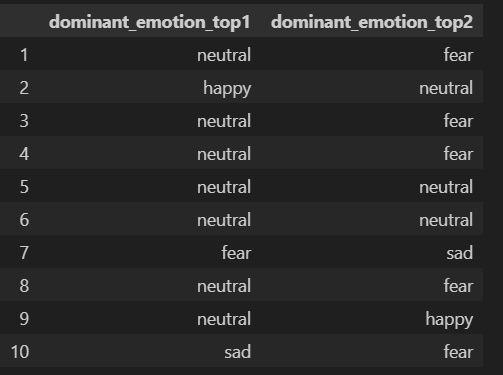
\includegraphics[width=1\columnwidth]{images_prompts/dominant_emotion.png}
\end{center}

\subsection{Integrating transcript data with emotion data}

\textbf{Prompt:}
\begin{tcolorbox}[title='Prompt']
    \lstinputlisting[language=Python]{prompts/trans_promt.txt}
\end{tcolorbox}
\begin{center}
    \color{red}\rule{1\linewidth}{0.5mm}
\end{center}

\begin{responsebox}
    The response from the chatgpt awesome this time.
\end{responsebox}

\begin{tcolorbox}
    \lstinputlisting[language=Python]{prompts/code2.txt}
\end{tcolorbox}

\large{Using above code, It extracted the above features of transcript data of each student and added to the final dataframe.}
\begin{center}
    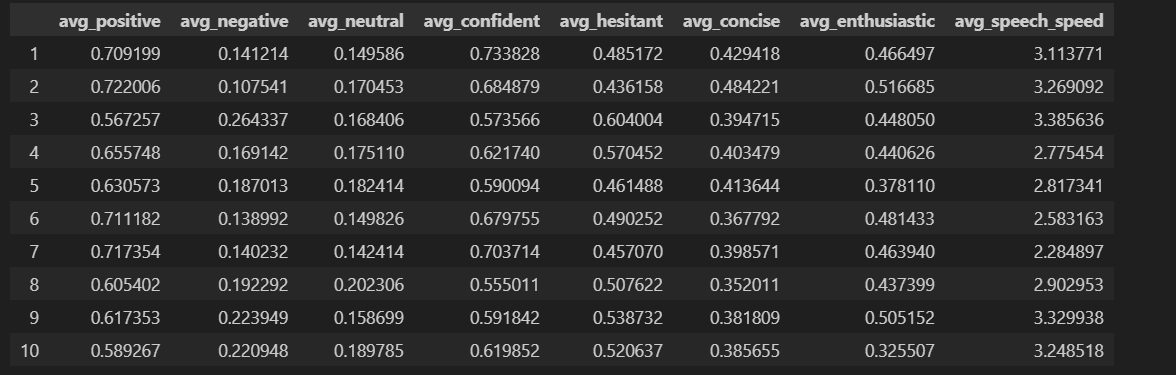
\includegraphics[width=1\columnwidth]{images_prompts/trans_df.png}
\end{center}

\begin{tcolorbox}[colback=yellow!10!white, colframe=red!80!black, title=Note]
  Now we have to merge the transcript data with the emotion data. \\
  For that we have to merge the dataframes on the basis of student id.
\end{tcolorbox}

\textbf{Prompt for merging the emotion\_df and transcript\_df:}
\begin{verbatim}[title=Prompt]
    df_dominantEmotion_for_everystudent
    and final_df add these df on index
\end{verbatim}
\begin{center}
    \color{red}\rule{1\linewidth}{0.5mm}
\end{center}

\text{response from the chatgpt:}
\begin{tcolorbox}
\begin{lstlisting}
final_df_with_emotions = pd.concat([final_df, df_dominantEmotion_for_everystudent], axis=1)

# Print the final merged DataFrame
print(final_df_with_emotions.head(10))

\end{lstlisting}
\end{tcolorbox}

\large{Using the above code, the emotion data and transcript data were merged on the basis of student id.}
\large{The final dataframe after merging the emotion and transcript data is shown below:}

\begin{tcolorbox}[colback=blue!5!white, colframe=green!70!black, title=Final Dataframe, fonttitle=\bfseries\Large]
\begin{tblr}{
    colspec = {lccccccccccc},
    row{1} = {font=\bfseries\color{red}},
    hlines,
    vlines,
    stretch = 0.1
}
\textbf{id} & \textbf{avg\_positive} & \textbf{avg\_negative} & \textbf{avg\_neutral} & \textbf{avg\_confident}  \\
1 & \textcolor{blue}{0.709199} & \textcolor{blue}{0.141214} & \textcolor{blue}{0.149586} & 0.733828 \\
2 & \textcolor{blue}{0.722006} & \textcolor{blue}{0.107541} & \textcolor{blue}{0.170453} & 0.684879 \\
\end{tblr}

\begin{tblr}{ colspec = {lccccccccccc},
    row{1} = {font=\bfseries\color{red}},
    hlines,
    vlines,
    stretch = 1}
\textbf{avg\_hesitant} & \textbf{avg\_concise} & \textbf{avg\_enthusiastic} & \textbf{avg\_speech\_speed} \\
0.485172 & 0.429418 & 0.466497 & 3.113771  \\
 0.436158 & 0.484221 & 0.516685 & 3.269092 \\
\end{tblr}
\begin{tblr}{ colspec = {lccccccccccc},
    row{1} = {font=\bfseries\color{red}},
    hlines,
    vlines,
    stretch = 1}

\textbf{dominant\_emotion\_top1} & \textbf{dominant\_emotion\_top2} \\
neutral & fear \\
happy & neutral \\
\end{tblr}
\end{tcolorbox}

\subsection{Now, Integrating the gaze\_df with the final\_df\_with\_emotions}
\begin{center}
    \color{red}\rule{1\linewidth}{1mm}
\end{center}
\textbf{But before that i have to extract the key features from all 10 gaze data and make a single gaze\_df.}
\textbf{Prompt for this:}
\begin{tcolorbox}
    \begin{lstlisting}
        i have gaze_df of 10 students 
in each csv of student there are 
	movie_id	image_seq	gaze	blink	eye_offset
0	93663f94-bf0a-4ce8-a29a-a5236cc7fe6a	1	1	0	6.2253
1	93663f94-bf0a-4ce8-a29a-a5236cc7fe6a	2	1	0	22.7274

data like this
now i want to make merged_gaze_df of all 10 students how can i do this?

    \end{lstlisting}
\end{tcolorbox}

\begin{center}
    \color{red}\rule{1\linewidth}{0.5mm}
\end{center}

\textbf{Response:}
\begin{tcolorbox}
I am just showing the code here. The whole response is \href{https://chatgpt.com/share/66eacd2e-b8f8-8009-8507-b3895c422e0b}{here}
    \begin{lstlisting}
# Read all 10 gaze CSV files and store them in a list
folder_path = 'emotion_data'
dfs= []
for i in range(1, 11):
    file_name = f'{i}/gaze.csv'
    file_path = os.path.join(folder_path, file_name)
    
    df = pd.read_csv(file_path)
    aggregated_df = df.groupby('movie_id').agg({
        'gaze': 'mean',          # Average gaze data over all frames
        'blink': 'sum',          # Total blinks across all frames
        'eye_offset': ['mean',   # Average eye_offset over the entire video
                        'max',    # Maximum eye_offset
                        'min',    # Minimum eye_offset
                        'std'],   # Standard deviation of eye_offset
        'image_seq': 'count'     # Count the number of frames
    }).reset_index()
    aggregated_df.columns = ['_'.join(col).strip() if isinstance(col, tuple) else col for col in aggregated_df.columns]
    dfs.append(aggregated_df)
    aggregated_df.head(2)

    
# print(dfs)

final_gaze_df = pd.concat(dfs)
\end{lstlisting}
\end{tcolorbox}
        

\section{Data Preprocessing}
\begin{center}
    \color{red}\rule{1\linewidth}{2mm}
\end{center}
\label{sec:preprocessing}

\textbf{Prompt:} "I have to check whether there are any missing values in the final DataFrame or not and also check the basic statistics of the final DataFrame."

\begin{tcolorbox}
    \begin{verbatim}

import os

folder_path = 'emotion_data'
#  if there is any data missing print the missing data
def check_dataframe(df):
    missing_values = df.isnull().sum()
    print("Missing values in each column:\n", missing_values)
    
    basic_statistics = df.describe()
    print("\nBasic statistics of the DataFrame:\n", basic_statistics)

for i in range(1, 11):
    file_name = f'{i}/emotion.csv'
    file_path = os.path.join(folder_path, file_name)
    
    if os.path.exists(file_path):
        df = pd.read_csv(file_path)
        print(f"Data from {file_path}:")
        check_dataframe(df)
    else:
        print(f"File {file_path} does not exist.")
    
    \end{verbatim}
\end{tcolorbox}

 from the results, i got following observations from the running this code:-
\begin{itemize}
    \item As the Count of all the features is 10, means there is not Null values.
    \item The standard devaition of all the features is also very low compared
    to the mean, indicating that the data is not spread out(low chances of
    outliers).
    \item As i have already done the encoding of the categorical features, so no
    need to do it again.
\end{itemize}


\section{Prompts for Analysis on the DataFrame made above}
\begin{center}
    \color{red}\rule{1\linewidth}{2mm}
\end{center}

\subsection{Basic Statistics}
\begin{center}
    \color{red}\rule{1\linewidth}{1mm}
\end{center}
\textbf{Prompt:}
\begin{tcolorbox}
    \begin{lstlisting}
     How to know whether there are any missing values in the final DataFrame?
     or just give me description of the dataframe.
    \end{lstlisting}
\end{tcolorbox}
\begin{center}
    \color{red}\rule{1\linewidth}{0.5mm}
\end{center}
\textbf{Response:}
\begin{tcolorbox}
    \begin{lstlisting}
    print(final_df_with_emotions.describe())
    \end{lstlisting}
\end{tcolorbox}

\large{The basic statistics of the final DataFrame are as follows:}
\begin{center}
    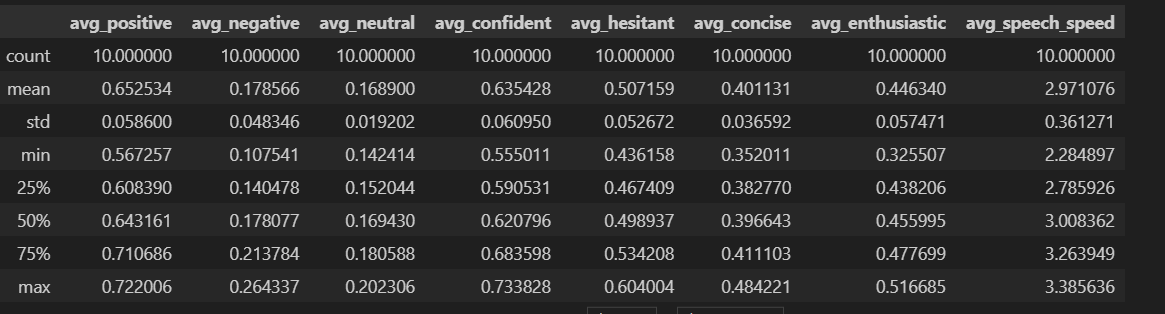
\includegraphics[width=1\columnwidth]{images_prompts/basic-stats.png}
\end{center}


\subsection{Correlation Analysis}
\begin{center}
    \color{red}\rule{1\linewidth}{1mm}
\end{center}
    Now i did correlation analysis on the final DataFrame to understand the relationship between different features.
\textbf{Prompt:}
\begin{tcolorbox}
    \begin{lstlisting}
    Now, calculate the correlation matrix of the final DataFrame final\_df.
\end{lstlisting}
\end{tcolorbox}
\begin{center}
    \color{red}\rule{1\linewidth}{0.5mm}
\end{center}
\textbf{Response:}
\begin{tcolorbox}
    \begin{lstlisting}
    correlation_matrix = final_df_with_emotions.corr()
    print(correlation_matrix)
    \end{lstlisting}
\end{tcolorbox}

\large{Wrtitng and running the code, there was a error in chatgpt response, but 
I corrected it and ran the code. The correlation matrix is shown below:}

\begin{center}
    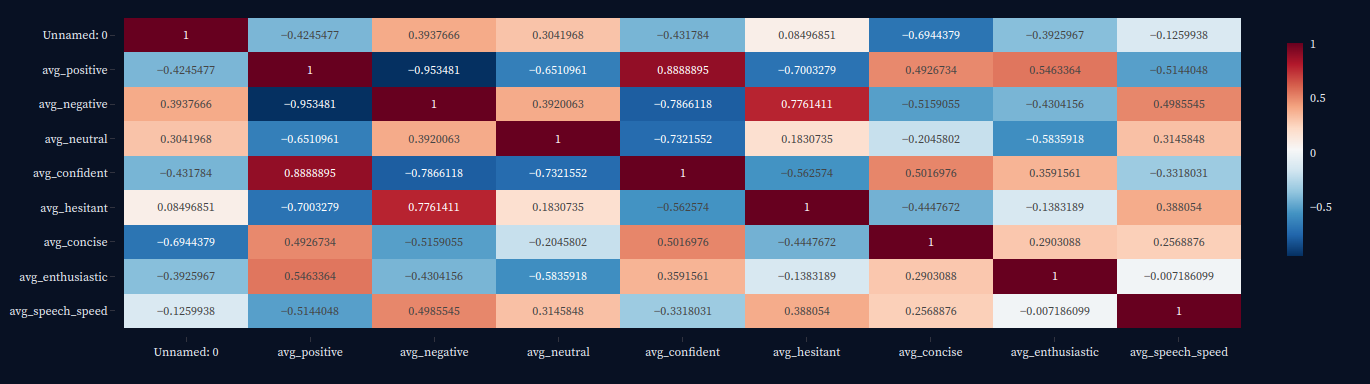
\includegraphics[width=1\columnwidth]{images/corr.png}
\end{center}

\subsection{Based on the final\_df, I asked for analysis on the data.}
\begin{center}
    \color{red}\rule{1\linewidth}{1mm}
\end{center}
\textbf{Prompt:}
\begin{tcolorbox}
  \lstinputlisting[language= python]{prompts/main.txt}
\end{tcolorbox}

\begin{center}
    \color{red}\rule{1\linewidth}{0.5mm}
\end{center}

\textbf{Response:}
\begin{tcolorbox}
   As the result of this response is very large, i am not pasting it here.
    But the link for the response is \href{https://chatgpt.com/share/66eac84c-2c84-800f-b800-e42a0607ce97}{here}
    But the crux of the response chatgpt is :
    \begin{enumerate}
        \item EDA Plots: Box plots, scatter plots, word clouds, heatmaps, and bar charts to visualize key metrics.
        \item Analysis: Emotional stability, communication skills, and expertise areas via correlation analysis, sentiment analysis, and text-based NLP.
        \item Recommendations: Tailored based on emotional and communication performance.
        \item Scoring Mechanism: Combine emotional stability, transcript quality, and communication clarity for ranking.
        \item Any Aditional insights
    \end{enumerate}
\end{tcolorbox}

\Large{So based on the response of the chatgpt, i started implementing each section one by one.}

\begin{tcolorbox}[colback=yellow!10!white, colframe=red!80!black, title=Note]
   In the responses, I am just showing the text response of the chatgpt. The code is not pasted here.\\
   I will expliclty include the code in different file or if the link for the chatgpt is mentioned, then \\
   no issues.
   If the response will be too long , i will just give what i understood from the response.\\
   and will paste the link for the response.
\end{tcolorbox}

\begin{itemize}
        \item Communication Scoring: {
            \textbf{Prompts for this section:}
            \begin{center}
                \color{red}\rule{1\linewidth}{0.5mm}
            \end{center}
            \begin{tcolorbox}
                \lstinputlisting[language=python]{prompts/comm.txt}
            \end{tcolorbox}
            \Large{In the response of this prompt, chatpgt gave codes for relations i wanted to find. I am not pasting the code here.
            Link for the chatgpt response is \href{https://chatgpt.com/share/66eac52b-9638-8009-aceb-bece7faa6be8}{here}}
            
        }
        \item Emotional State and Body Language Analysis: {
            \textbf{Prompts for this section:}
            \begin{center}
                \color{red}\rule{1\linewidth}{0.5mm}
            \end{center}
            \begin{tcolorbox}[title=Prompt]
                \lstinputlisting[language=python]{prompts/emotion.txt}
            \end{tcolorbox}
            \begin{center}
                \color{red}\rule{1\linewidth}{0.5mm}
            \end{center}
            \begin{center}
                \color{red}\rule{1\linewidth}{0.5mm}
            \end{center}
            \textbf{Response:}

            \begin{tcolorbox}[title=Response]
                \lstinputlisting{prompts/emotion-res.md}
            \end{tcolorbox}
            \begin{center}
                \color{red}\rule{1\linewidth}{0.5mm}
            \end{center}
            \textbf{Further Prompts for this section:}
            \begin{tcolorbox}[title= prompt]
                what is eye-offset can u explain??
            \end{tcolorbox}
         
            \begin{center}
                \color{red}\rule{1\linewidth}{0.5mm}
            \end{center}
            \textbf{Response:}
            \begin{tcolorbox}[title= response]
                \begin{lstlisting}
Eye offset is the distance between the center of the screen and the point where the user is looking. 
It is used to measure the stability of the user's gaze. 
A higher eye offset indicates that the user's gaze is less stable.
                \end{lstlisting}
            \end{tcolorbox}



\begin{tcolorbox}[title= Prompts for analysing gaze\_df:]
\begin{lstlisting}
No, i want U to give Eye Offset Standard Deviation analysis for every student on the basis of 
1.Too much Eye Movements:
2. Moderate Eye Movements:
3. Stable Eye Movements:
\end{lstlisting}
\end{tcolorbox}
\begin{center}
    \color{red}\rule{1\linewidth}{0.5mm}
\end{center}
\begin{tcolorbox}[title=response]
    As the response is very long, i am not pasting it here.\\
    The link for the response is \href{https://chatgpt.com/share/66eacd2e-b8f8-8009-8507-b3895c422e0b}{here}

    But the summary of the response is:
    \begin{enumerate}
        \item Group data by student: Calculate the standard deviation of eye_offset for each student across all video frames.
        \item Define thresholds for categorizing the movements into:{
            \begin{itemize}
                \item Too much Eye Movements: High standard deviation.
                \item Moderate Eye Movements: Medium range of standard deviation.
                \item Stable Eye Movements: Low standard deviation.
            \end{itemize}
        \item Categorize each student based on their standard deviation.
        }
    \end{enumerate}

\end{tcolorbox}
    
        }
    \end{itemize}

  
\section{Scoring of the Students based on the data.}
\textbf{Prompt:}
\begin{center}
    \color{red}\rule{1\linewidth}{0.5mm}
\end{center}
\large{So i had already some latex code, on that i asked chatgpt to give me the scoring mechanism for the students based on the data.}
\Large{So my prompt was like this:}

\begin{tcolorbox}[title= response]
    \begin{lstlisting}
based on the data, do the changes in the latex also provide insights acc to the data 
and comparison with other students (ranking in every feature), and use tcolorbox for heading only.
    \end{lstlisting}
\end{tcolorbox}
\textbf{Response:}
\large{The response of the chatgpt was NOTvery good. It gave me the scoring mechanism just on the basis of few features.}


\textbf{Refined Prompt:}

\begin{tcolorbox}[title=Refined Prompt]
    \begin{lstlisting}
Analysis the data deeply and on the basis of all the features of each student, give a scoring mechanism such that
1) It is robust
2) divides the student into highly fit for the role
3) Okk for the role
4) Not for the role
5) Main focus should be on transcript data(postive,negative,neutral) , emotion thorughtout the video, confidence, hesitance, speech,speed, body language, enthusiam
    \end{lstlisting}
\end{tcolorbox}
\begin{center}
    \color{red}\rule{1\linewidth}{0.5mm}
\end{center}


\textbf{Response:}
This time, response was amazing, it gave a very nice framework to calculate and rank the students based on the data.\\
Though values used for the scoring were random, but the framework was very good.\\

\begin{tcolorbox}[title=Response]
    \lstinputlisting[language=python]{prompts/score.txt}
\end{tcolorbox}

\Large{This was the original response, here values used for the scoring and weightwage were not good. So i changed them.}

\Large{To see complete prompts and responses(including wrong one), click \href{https://chatgpt.com/share/66eac84c-2c84-800f-b800-e42a0607ce97}{here}}

% Additional sections continue in a similar format...



\section{Conclusion}
\label{sec:conclusion}
This section summarizes the key findings and insights from the data analysis project.
% based on the whole latex code above , give the conclusion of the project in words.
\begin{center}
    \color{red}\rule{1\linewidth}{1mm}
\end{center}
\textbf{Prompt:}

\begin{tcolorbox}[title=Prompt]
    \begin{lstlisting}
        Based on the analysis of the data, provide a conclusion for the project. 
        Include key insights, recommendations, and any additional observations.
    \end{lstlisting}
\end{tcolorbox}

\begin{center}
    \color{red}\rule{1\linewidth}{0.5mm}
\end{center}

\textbf{Response:}
\begin{tcolorbox}[title=Response]
    \begin{lstlisting}
        Based on the analysis of the data, the following conclusions can be drawn:
        1. Students with high positive sentiment, confidence, and enthusiasm are more likely to be successful in the role.
        2. Communication skills, including concise speech and moderate speech speed, are important for effective communication.
        3. Emotional stability and body language play a significant role in conveying confidence and enthusiasm.
        4. Students with stable eye movements and low eye offset are more likely to maintain focus and attention.
        5. Recommendations: Provide training in emotional intelligence, communication skills, and body language to improve student performance.
        6. Additional observations: The scoring mechanism can be further refined based on additional data and feedback from experts.
    \end{lstlisting}
\end{tcolorbox}

\vfill

\begin{center}
    
\includegraphics[width=1\columnwidth]{images/thank.png}
\end{center}
\vfill
% References
\bibliographystyle{plain}
\bibliography{references}

\end{document}